\documentclass[letterpaper]{article}
\usepackage[utf8]{inputenc}
\usepackage[spanish,es-lcroman]{babel}
\usepackage{fancyhdr}
\usepackage{lastpage}
\usepackage{extramarks}
\usepackage{graphicx}
\usepackage{float}
\usepackage{amsmath}
\usepackage{hyperref}
\usepackage{booktabs}
\usepackage[usenames,dvipsnames]{xcolor}
\usepackage{listings}


% Margenes
\topmargin=-0.45in
\evensidemargin=0in
\oddsidemargin=0in
\textwidth=6.5in
\textheight=9.0in
\headsep=0.25in


% Header y footer
\pagestyle{fancy}
\lhead{}
\chead{\guiaRamo\: \guiaTitulo} % Centro
\rhead{2015.2}
\lfoot{UTFSM-CSJ}
\cfoot{}
\rfoot{Página\ \thepage\ de\ \protect\pageref{LastPage}} % Pagina
\renewcommand\headrulewidth{0.4pt}
\renewcommand\footrulewidth{0.4pt}


% Syntax Highlight
\lstdefinestyle{basic} {
  basicstyle=\footnotesize\ttfamily,
  numbers=left,
  numberstyle=\footnotesize\color{cyan}\ttfamily,
  numbersep=5pt,
  frame=tb,
  rulecolor=\color{cyan},
  captionpos=t,
  keywordstyle=\color{blue},
  breaklines=true,
  commentstyle=\color{gray},
  columns=fullflexible,
  stringstyle=\color{Purple}
}
\newcommand{\python}[2]{
    \begin{itemize}
        \item[]\lstinputlisting[style=basic,language=python,caption=#2,label=#1]{#1}
    \end{itemize}
}
\lstset{
  literate={ó}{{\'o}}1
           {á}{{\'a}}1
           {ú}{{\'u}}1
           {í}{{\'i}}1
           {é}{{\'e}}1
}


\makeatletter
\newcommand{\titulo}[2]{%
  \vspace{#2}\noindent{#1}\vspace{\baselineskip}%
  \@afterindentfalse\@afterheading}
\makeatother




%------------------------------------------------------------------------
%	Meta Información
%------------------------------------------------------------------------
\newcommand{\guiaTitulo}{Tarea 2-3} % titulo del informe
\newcommand{\guiaFecha}{\today} % Fecha
\newcommand{\guiaRamo}{Seminario de Modelos y Métodos Cuantitativos} % Ramo
\newcommand{\guiaIniciales}{AL,JPEG} % Ramo
\newcommand{\guiaProfesor}{Andrés Moreira} % Profesor

%------------------------------------------------------------------------
%	Título
%------------------------------------------------------------------------
\title{
    \textmd{\textbf{\guiaRamo\\ \guiaTitulo}}\\
    \vspace{0.1in}
    \large{\textsc{Universidad Técnica Federico Santa María - Campus San Joaquín}}\\
    \normalsize\vspace{0.1in}\small{\guiaFecha}\\
    \vspace{0.1in}\large{\textit{Profesor \guiaProfesor}}
}
\author{
    \textsc{Juan Pablo Escalona G.} \\
    \small{juan.escalonag@alumnos.usm.cl} \\
    {\small 201073515-k}
    \and
     \textsc{Alonso Lepe M.} \\
    \small{alonso.lepe@alumnos.usm.cl}\\
    {\small 201173593-5}
\vspace{.5in}
}
\date{}

\begin{document}

\maketitle
\section{Pregunta 1}
Se tiene un grafo $G(n=400,p=1)$ esto implica que hay 79800 aristas que conectan a los 400 nodos entre todos. i.e. $\frac{399 \cdot 400}{2} = 79800$

Para que una componente conexa sea gigante debe tener un $k = np > 1$, en este caso $k = 400$, como se necesita un $k <= 1$ para que deje de ser gigante, entonces $p$ debería ser a lo mas $\frac{1}{400} = 0.0025$

Si se elimina una arista en el segundo 00:00:01 entonces aún quedan 79799 aristas, es decir, una probabilidad de $p = \frac{79799}{79800} = 0.9999$. Pero se sabe que se necesita una probabilidad de 0.0025, por lo que la componente dejará de ser conexa cuando solo hayan $\frac{E}{79800} = 0.0025 \implies E \sim 200$ aristas.

Luego si cada segundo se elimina 1 arista y es preciso eliminar 79600 aristas entonces se tendría que esperar hasta las 22:06:40 (10 de la noche, 6 minutos y 40 segundos)

Sobre este análisis se realizó el código \ref{codigos/p1.py} del anexo en el que se crea una red ER de 400 nodos y probabilidad 1. Luego se comenzó a eliminar nodos hasta lograr un grado promedio < 1. Se ejecutó el código en un computador con un 2.5 GHz Intel Core i5 y 8 GB ram, tardó 8 minutos 29 segundos en eliminar aristas hasta lograr un grado promedio de 1. Finalmente se eliminaron 79600 aristas por lo que empíricamente también terminó a las 22:06:40

\section{Pregunta 2}
La Matriz laplaciana de un grafo se puede obtener a partir de la matriz de adyacencia siguiendo el siguiente formato:
\begin{align}
  l_{i,j} =
  \begin{cases}
    k_i  & \text{si } i = j  \\
    -1  & \text{si } i \neq j  \\
    0  & \text{e.t.o.c.}
  \end{cases}
\end{align}

que es lo mismo que decir $l = K - A$ donde K es la matriz diagonal de los grados de cada nodo y A es la matriz de adyacencia. Luego para la matriz de adyacencia dada se tiene la siguiente matriz laplaciana:

\begin{align}
l = \begin{bmatrix}
   2  &-1  &-1  & 0  & 0  & 0    \\
   -1 &  2 & -1 &  0 &  0 &  0   \\
   -1 & -1 &  3 & -1 &  0 &  0   \\
    0 &  0 & -1 &  3 & -1 & -1   \\
    0 &  0 &  0 & -1 &  2 & -1   \\
    0 &  0 &  0 & -1 & -1 &  2
\end{bmatrix}
\end{align}

l valor de Fiedler es el segundo valor propio mas pequeño, en este caso corresponde a 0.438 ubicado en la tercera columna como se muestra en las ecuaciones (\ref{eq:fiedler1}) y (\ref{eq:fiedler2}).


\begin{align}
  V &= \begin{bmatrix}
     0.185 & -0.408 & \textbf{ 0.465} &  0.378 & -0.756 &  0.040 \\
     0.185 & -0.408 & \textbf{ 0.465} & -0.734 &  0.463 &  0.238 \\
    -0.657 & -0.408 & \textbf{ 0.261} &  0.357 &  0.292 & -0.278 \\
     0.657 & -0.408 & \textbf{-0.261} &  0.357 &  0.292 & -0.278 \\
    -0.185 & -0.408 & \textbf{-0.465} & -0.189 & -0.148 & -0.472 \\
    -0.185 & -0.408 & \textbf{-0.465} & -0.168 & -0.145 &  0.751
  \end{bmatrix} \label{eq:fiedler1}\\
  E &= \begin{bmatrix} \quad 4.562 & \quad 0.000 & \; \textbf{0.438} & \quad 3.000 & \; \; 3.000 & \;\;\; 3.000 \end{bmatrix} \label{eq:fiedler2}
\end{align}

Es importante ordenarlos para obtener el valor de Fiedler, pues este es el segundo menor valor propio.
\begin{align}
  \text{Valor de Fiedler: }  & \; 0.4384\\
  \text{Vector de Fiedler: } & \begin{bmatrix}0.465 & 0.465 & 0.261 & -0.261 & -0.465 & -0.465\end{bmatrix}
\end{align}


\begin{figure}[H]
  \centering
  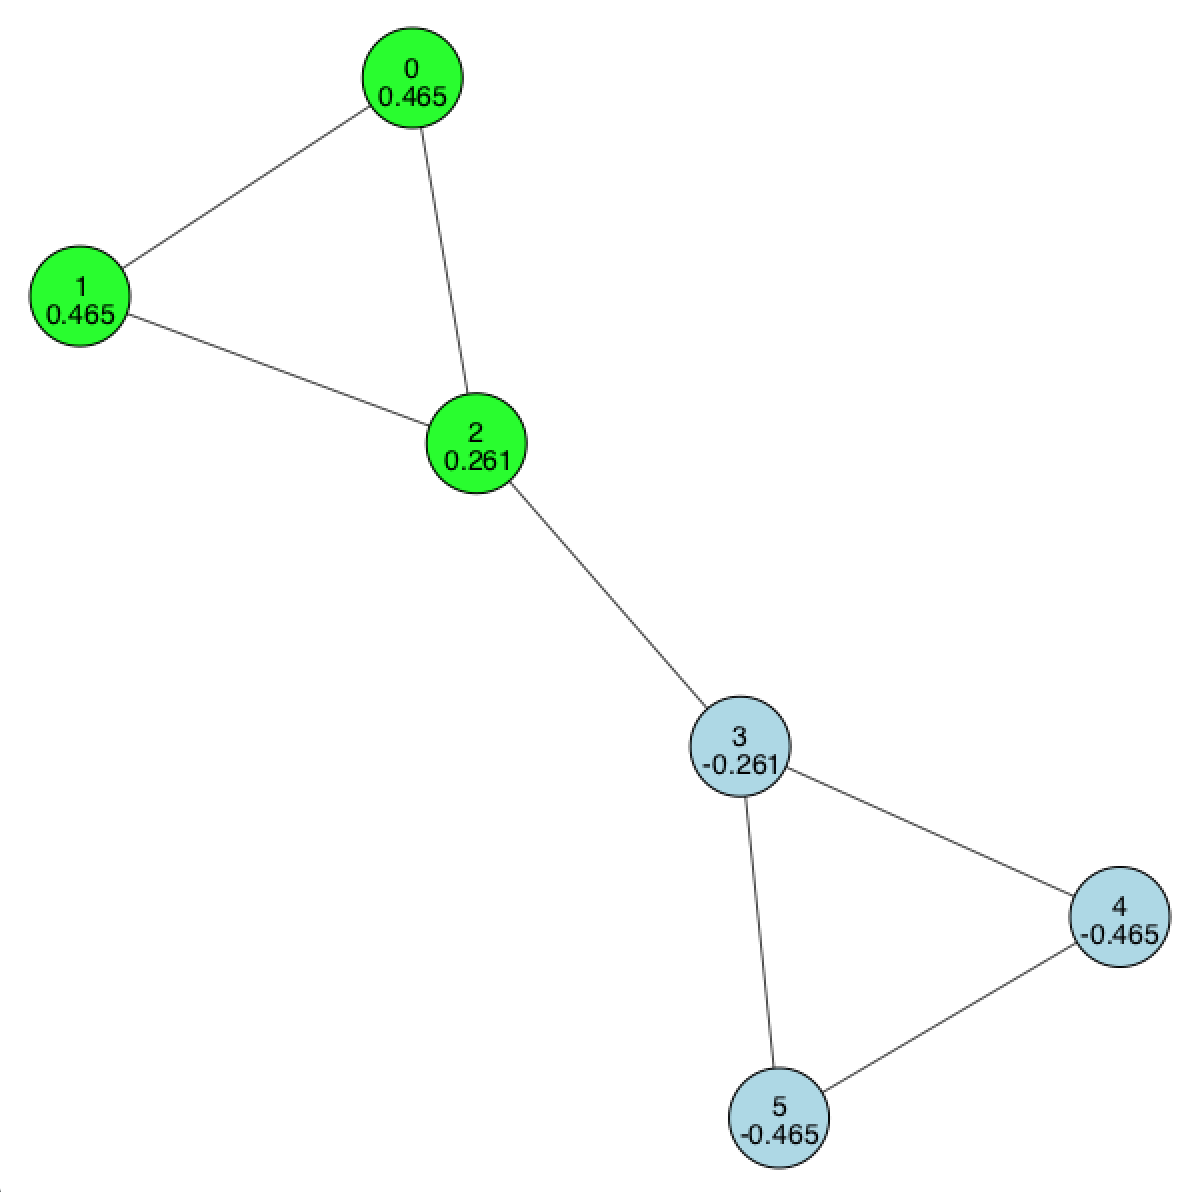
\includegraphics[width=.7\linewidth]{img/p2.png}
  \caption{Partición de la red en dos comunidades mostrando sus respectivos valores del vector propio.}
  \label{red:2}
\end{figure}

Se decidió cortar en el 0, pues los valores se separan uniformemente en torno al este. Se observan claramente dos comunidades en esta red las que interactúan únicamente por el vértice 2-3.





\section{Pregunta 3}
Dos nodos de un grafo forman un \textit{2-componente} si existen al menos dos caminos independientes entre ellos. Un camino es una secuencia finita de aristas que permiten ir de un nodo inicial a un nodo final dentro de un grafo.

Un \textit{2-componente} o \textit{biconnected component} tienen la particularidad que si se elimina una arista del grafo, aún sería posible llegar de un nodo a otro, pues originalmente existían dos posibles caminos.

Por otro lado un \textit{2-core} es un conjunto de nodos donde cada uno está conectado a los demás con al menos 2 aristas. Un \textit{2-core} solo considera los nodos que estén conectados con una arista dentro del conjunto, si algún nodo tiene una arista a un nodo fuera del conjunto, dicha arista no se cuenta.



\begin{figure}[H]
  \centering
  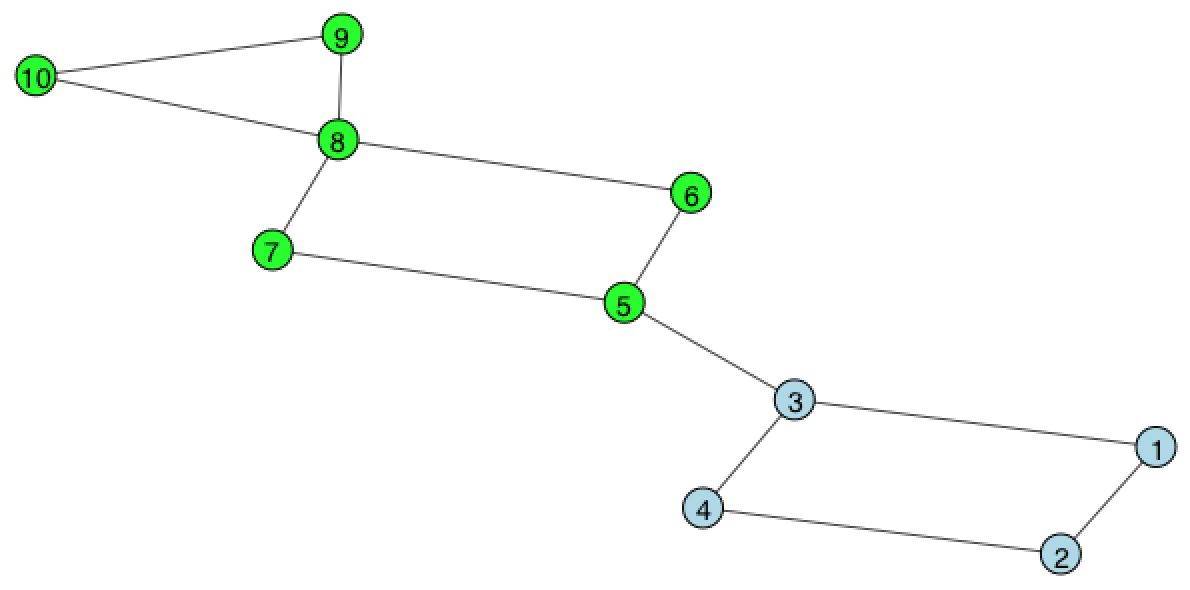
\includegraphics[width=.6\linewidth]{img/p3.png}
  \caption{ Grafo 2-core con dos 2-componentes.}
  \label{red:3}
\end{figure}

En la figura \ref{red:3} se aprecia un grafo con un solo conjunto \textit{2-core} con la totalidad de los nodos, pues todos los nodos del grafo están conectados a los demás con al menos 2 aristas.

Por otra parte existen dos \textit{2-componentes} destacados por los colores. En este caso el \textit{2-componente} $\left[1,2,3,4\right]$ y el componente $\left[5,6,7,8,9,10\right]$. No puede existir un 2-componente entre el nodo 1 y el nodo 8, pues si o si hay que pasar por la arista 3-5 por lo que sería el mismo camino. Si se quita dicha arista no hay otra forma de llegar de 1 a 8.


\section{Pregunta 4}

\subsection{Grafico de la red}
\begin{figure}[H]
  \centering
  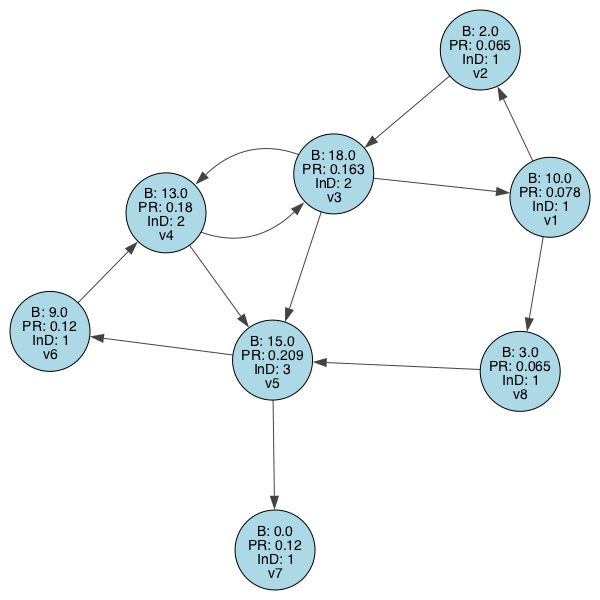
\includegraphics[width=.5\linewidth]{img/p4-all.png}
  \caption{Red chica dirigida. B: Betweenness, PR: PageRank, InD: Grado de entrada.}
  \label{red:4}
\end{figure}

\begin{figure}[H]
  \centering
  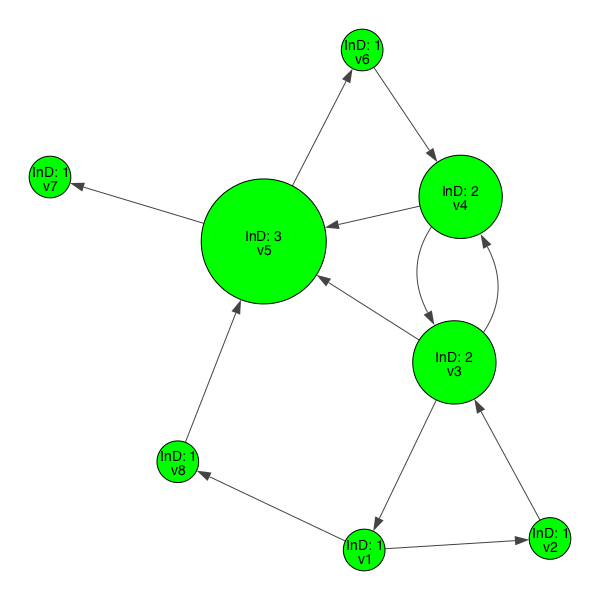
\includegraphics[width=.32\linewidth]{img/p4-indegree.png}\hfill
  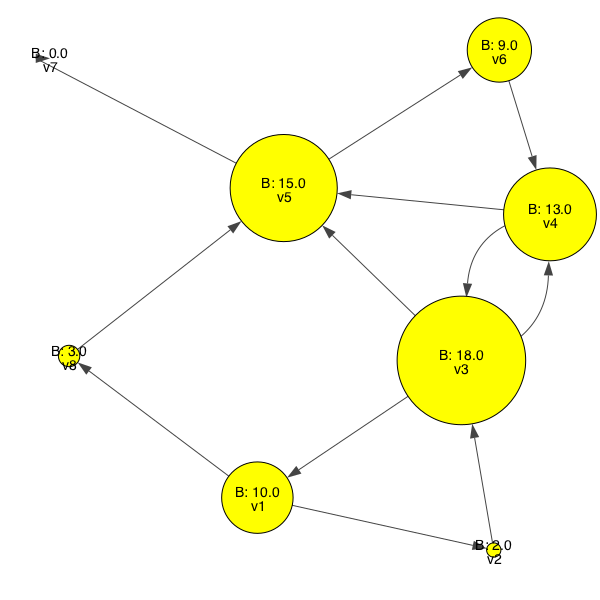
\includegraphics[width=.32\linewidth]{img/p4-betweenness.png}\hfill
  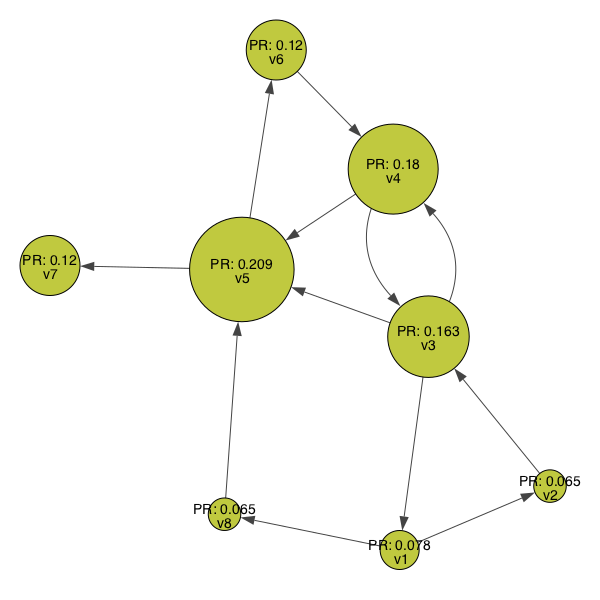
\includegraphics[width=.32\linewidth]{img/p4-pageranks.png}
  \caption{Red chica según el tamaño porcentual para cada indice.}
  \label{red:4-all}
\end{figure}



\subsection{Ranking de los índices}
\begin{table}[H]
  \centering
  \renewcommand{\arraystretch}{1.1}
  \begin{tabular}{@{}ccccccccccc@{}}
    \toprule
       \multicolumn{3}{c}{\textsc{Grado Entrada}} & \phantom{abc} & \multicolumn{3}{c}{\textsc{Betweenness}} & \phantom{abc} & \multicolumn{3}{c}{\textsc{PageRank}}\\
       \cmidrule{1-3}\cmidrule{5-7}\cmidrule{9-11}
       Posición & Nodo & Valor & & Posición & Nodo & Valor & & Posición & Nodo & Valor\\
       \midrule
      1 & v5 & 3 &&  1 & v3 & 18 && 1 & v5 & 0.209 \\
      2 & v4 & 2 &&  2 & v5 & 15 && 2 & v4 & 0.180 \\
      2 & v3 & 2 &&  3 & v4 & 13 && 3 & v3 & 0.163 \\
      3 & v1 & 1 &&  4 & v1 & 10 && 4 & v6 & 0.120 \\
      3 & v2 & 1 &&  5 & v6 & 9  && 4 & v7 & 0.120 \\
      3 & v6 & 1 &&  6 & v8 & 3  && 5 & v1 & 0.078 \\
      3 & v7 & 1 &&  7 & v2 & 2  && 6 & v2 & 0.065 \\
      3 & v8 & 1 &&  8 & v7 & 0  && 6 & v8 & 0.065 \\
    \bottomrule
  \end{tabular}
  \caption{Ranking de cada índice para la red chica.}
  \label{table:1}
\end{table}
Lo más evidente que se observa del Cuadro \ref{table:1} asi como también en la Figura \ref{red:4-all} es que los nodos v3, v4 y v5 están siempre en los primeros 3 puestos sin excepción, i.e. tienden a ser los nodos más relevantes de la red independiente del índice que se utilice para rankearlos.

Un aspecto interesante es la importancia del nodo v7, en el caso del grado de entrada el nodo v7 tiene solo 1 nodo de entrada por lo que su importancia es pequeña, en PageRank por otro lado tiene un nodo de entrada, pero esta arista proviene del nodo más importante de la red por lo que v7 adquiere una mayor importancia que los otros nodos que solo tienen grado de entrada 1.

Curiosamente el betweenness del nodo v7 es el más pequeño de todos en dicho ranking, pues no existen caminos que pasen por el. Es una importante diferencia entre Betweenness y PageRank. PageRank considera la importancia de un nodo según la importancia del nodo desde donde se llega, más aún si el enlace es mutuo, esto por la frecuencia con que se visitará dicho nodo al azar. Betweenness al contrario solo considera la cantidad de caminos que utilizan dicho nodo.

El más simple de todos es el grado de entrada, se observa que es muy similar al resultado obtenido en PageRank, pero PageRank le da más importancia a aquellos que llegan de un nodo importante, no solo de la cantidad de referencias que tenga.

El nodo v1 es muy similar en grado de entrada y PageRank, pero betweenness le asigna una gran importancia, siendo que tan solo tiene 1 grade de entrada, esto se podría explicar por la cantidad de caminos que permite construir ya que tiene dos aristas de salida, parece ser que tendría un gran flujo, menor que su predecesor el nodo v3.
\section{Pregunta 5}

Para esta pregunta se programaron los scripts \ref{codigos/p5-1-gnutella.py}, \ref{codigos/p5-2-delfines.py}, \ref{codigos/p5-3-erdos-renyi-gnutella.py} y \ref{codigos/p5-4-erdos-renyi-delfines.py}. En cada caso se carga una red diferente, gnutella, delfines y Erdös-Renyi. Luego para cada red se eliminan los nodos al azar, en orden decreciente de grado y en orden decreciente de betweenness. Luego se calcula el porcentaje de nodos que fue necesario eliminar para que el tamaño de la componente gigante se disminuyera a la mitad.

\begin{table}[H]
  \centering
  \renewcommand{\arraystretch}{1.1}
  \begin{tabular}{@{}lcccc@{}}
    \toprule
       Red & Azar & Grado Decreciente & Betweenness Decreciente\\
       \midrule
       \textsc{Gnutella} & 33.208\% &  3.019\% &  3.145\% \\
       \textsc{Delfines} & 38.710\% & 24.194\% & 12.903\% \\
       \textsc{Erdös-Renyi Gnutella} & 30.566\% & 9.128\% & 5.786\% \\
       \textsc{Erdös-Renyi Delfines} & 46.774\% & 32.258\% & 27.419\% \\

    \bottomrule
  \end{tabular}
  \caption{Porcentaje de nodos eliminados para cada red y para cada heurística de eliminación. Los valores al azar y las redes Erdös-Renyi son el promedio de 25 ejecuciones cada uno.}
  \label{table:2}
\end{table}

La red \textsc{gnutella} está compuesta de 795 nodos y 852 aristas mientras que la red \textsc{delfines} está compuesta por 62 nodos y 159 aristas. Para ambas redes se realizó una ER con la misma cantidad de nodos y aristas para comparar.

El resultado general mas destacable es que eliminar nodos al azar no es un buen método de reducción de componentes gigantes, pues la cantidad de nodos necesarios a eliminar variaba entre un 30\% y un 47\%, valores muy elevados, pues se está eliminando casi la mitad de la red para deshacerse de la componente gigante.

Por el contrario el método que presenta los mejores resultados tiene ser el de eliminación por betweenness decreciente. Para redes grandes como \textsc{gnutella} basta eliminar solo el 3.145\%, un valor similar fue necesario para la ER correspondiente.

El método del grado decreciente se comporta bien en redes grandes al igual que el método de betweennes. Ambos métodos caen en redes mas pequeñas como la de \textsc{delfines}, en donde se tiene que eliminar 24.193\% de los nodos con el método del grado y 12.903\% en el caso del betweenness. Estos valores altos se replican en la ER correspondiente a delfines, en donde para todos los métodos se tienen valores superiores a los 27\%.

\section{Pregunta 9}

\subsection*{(a)}
Para este experimento se utilizó la red ``pescado.gml'' y se pretende hallar reciprocidad corregida de la red. Para esto se procedió a encontrar la siguiente expresión:

\begin{align}
  \rho = \frac{\rho_1 - \bar{a}}{1 - \bar{a}}
\end{align}
en donde
\begin{align}
  \rho_1 &= \frac{1}{m}\sum_{i \neq j} a_{ij}a_{ji} \\
  \bar{a} &= \frac{1}{n(n-1)}\sum_{i \neq j} a_{ij}
\end{align}
los valores encontrados fueron
\begin{itemize}
  \item $\rho_1  =  0.4672$
  \item $\bar{a} = 0.1211$
\end{itemize}
luego $\rho = 0.3938 > 0$ lo que implica que la red presenta reciprocidad, la reciprocidad mide la tendencia de pares de nodos para formar conexiones mutuas entre ellos. En este caso se tiene una tendencia $\rho = 0.3938$ a formar conexiones mutuas entre pares de nodos, lo cual tiene sentido para el comercio e intercambio de pescado entre naciones.

\subsection*{(b)}
Ahora se procede a realizar un histograma para el peso total que entra a cada nodo y el peso total que sale de un nodo. Para esto basta con calcular la suma de las filas o columnas de la matriz de adyacencia con pesos. Esto luego se plotea como histograma, los resultados se adjuntan en la Figura~\ref{chart:1}.

Inmediatamente se reconoce en ambas distribuciones una ley de potencia, hay unos pocos que tienen mucho, y hay muchos que tienen muy poco. Para hallar las ecuaciones correspondientes a cada distribución se utilizo excel para realizar la regresión potencial correspondiente dado los valores entregados por la función de histograma en matplotlib.

\begin{figure}[H]
  \centering
  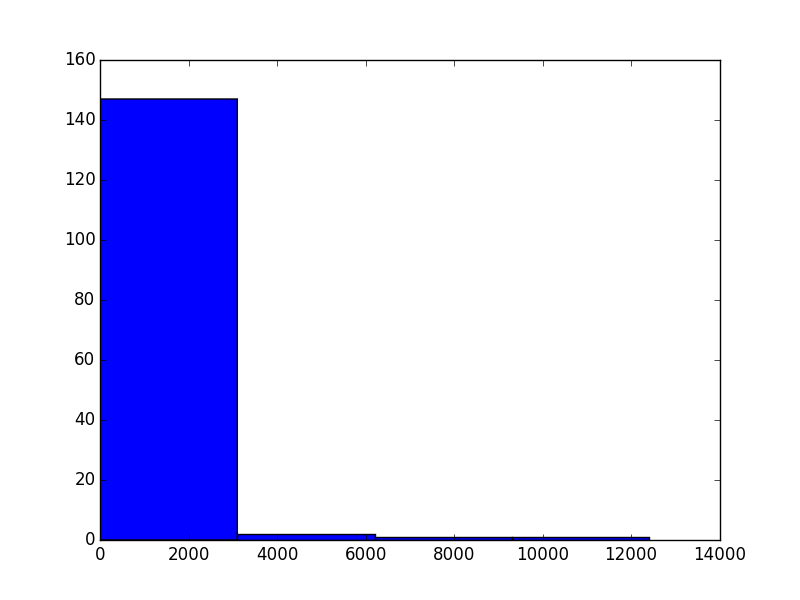
\includegraphics[width=.49\linewidth]{img/p9-s-in.png}\hfill
  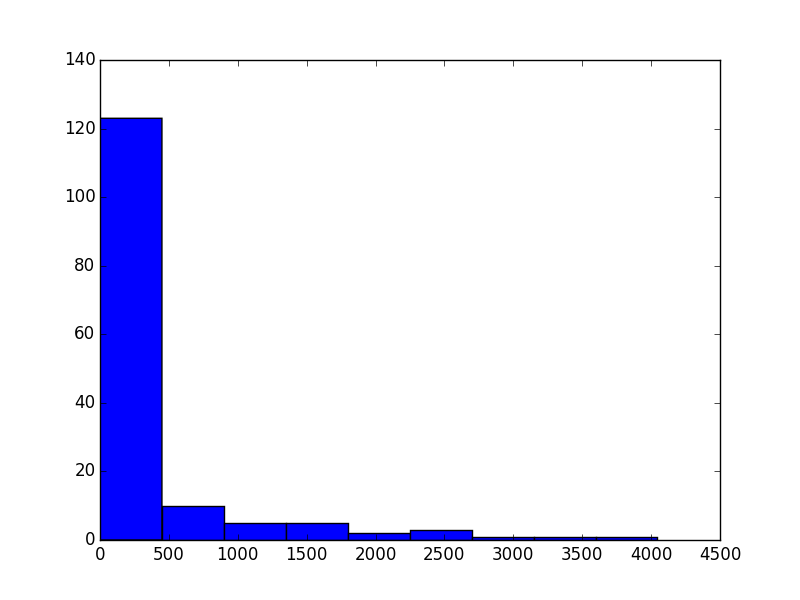
\includegraphics[width=.49\linewidth]{img/p9-s-out.png}\hfill
  \caption{Histogramas para $S^{in}$ y $S^{out}$ respectiamente.}
  \label{chart:1}
\end{figure}
Las expresiones encontradas fueron:
\begin{align}
  f^{in}(x)  &= 79.673\cdot x^{-3.722} & \qquad R^2 = 0.86766 \\
  f^{out}(x) &= 73.115\cdot x^{-2.07}  & \qquad R^2 = 0.93403
\end{align}

\subsection*{(c)}
En este experimento se intenta hallar alguna relación entre la suma de los pesos de los arcos que entran y salen de un nodo. Para esto se realiza el gráfico \ref{chart:2}
\begin{figure}[H]
  \centering
  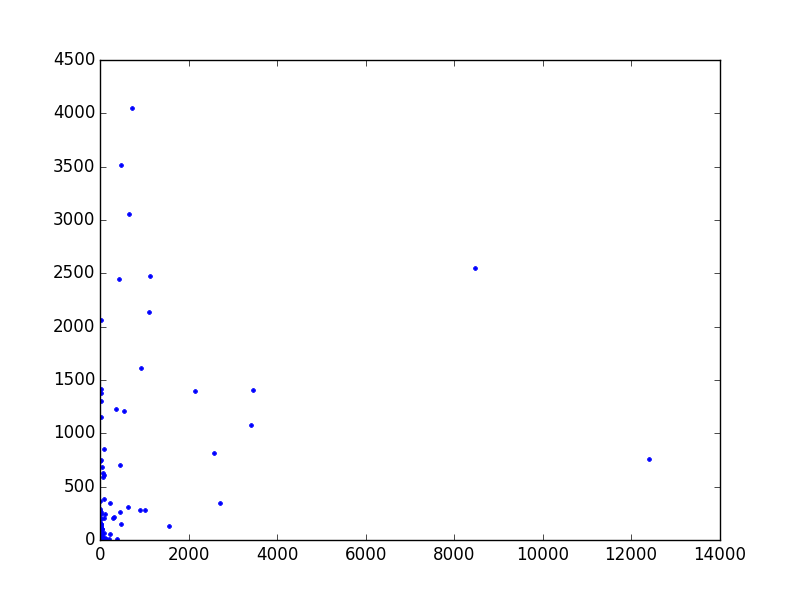
\includegraphics[width=.75\linewidth]{img/p9-s-s.png}\hfill
  \caption{$S^{in}$ vs $S^{out}$}
  \label{chart:2}
\end{figure}

En este gráfico no se observa ninguna relación entre las variables, i.e. no hay relación entre la cantidad de pescado importado y exportado en un país.

\subsection*{(d)}
Ahora se trabaja con el grafo no dirigido en que las aristas son la suma de los pesos del grafo dirigido anterior.
\begin{figure}[H]
  \centering
  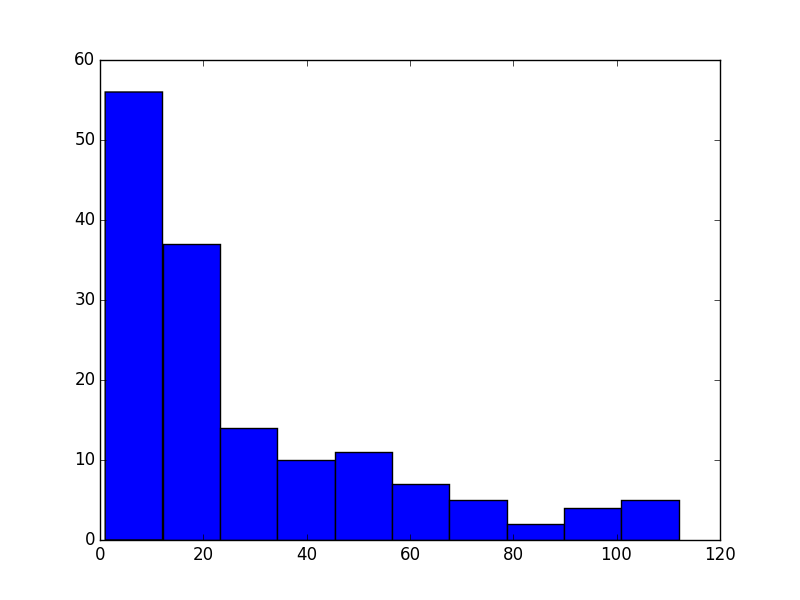
\includegraphics[width=.49\linewidth]{img/p9-k.png}\hfill
  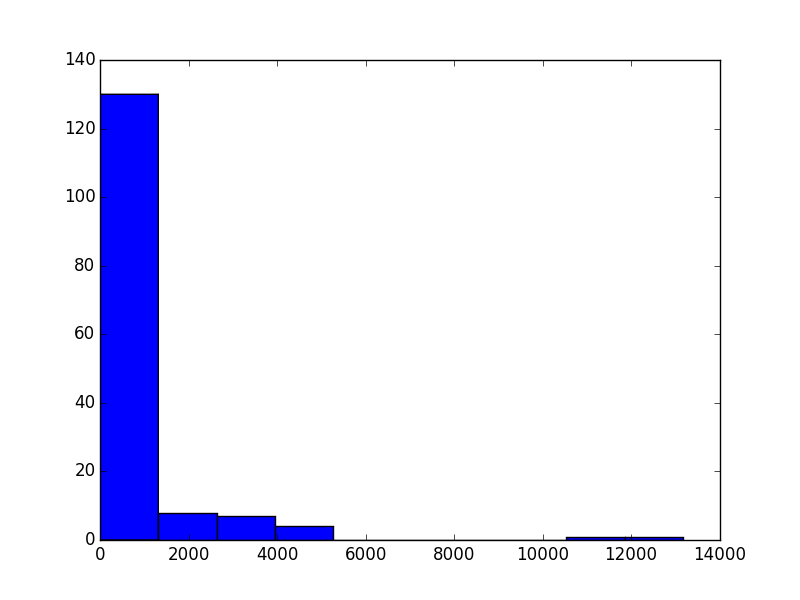
\includegraphics[width=.49\linewidth]{img/p9-s.png}\hfill
  \caption{Histogramas para P(k), P(s)}
  \label{chart:3}
\end{figure}
En este caso se hallan nuevamente leyes de potencia. Las expresiones halladas fueron:


\subsection*{(e)}

\begin{figure}[H]
  \centering
  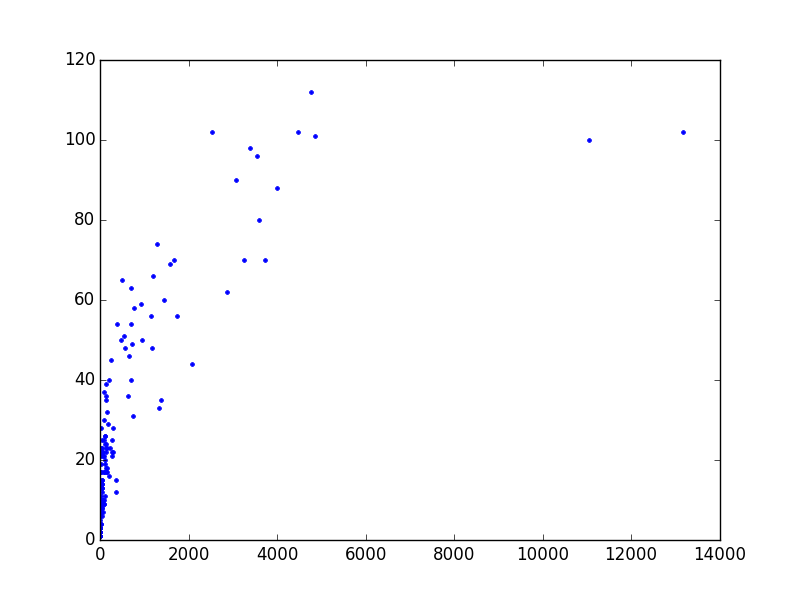
\includegraphics[width=.75\linewidth]{img/p9-k-vs-s.png}
  \caption{Grado vs fuerza de los nodos.}
  \label{chart:4}
\end{figure}

En este caso se observa una ley de potencia positiva, de este grafico se obtuvo la siguiente expresión:

\begin{align}
f(x) &= 2.5736x^{0.4313} & \qquad R^{2} = 0.87075
\end{align}

el $R^2$ indica la presencia de una buena relación entre las variables.


\section{Referencias}
\section{Apéndice}

\python{codigos/p1.py}{p1.py}
\python{codigos/p2.py}{p2.py}
\python{codigos/p3.py}{p3.py}
\python{codigos/p4.py}{p4.py}
\python{codigos/p5-1-gnutella.py}{p5-1-gnutella.py}
\python{codigos/p5-2-delfines.py}{p5-2-delfines.py}
\python{codigos/p5-3-erdos-renyi-gnutella.py}{p5-3-erdos-renyi-gnutella.py}
\python{codigos/p5-4-erdos-renyi-delfines.py}{p5-3-erdos-renyi-delfines.py}


\end{document}
